%----------------------------------------------------------------------------------------
%	PACKAGES AND THEMES
%----------------------------------------------------------------------------------------
\documentclass[aspectratio=169,xcolor=dvipsnames]{beamer}
\usetheme{Simple}

\usepackage{hyperref}
\usepackage{graphicx} % Allows including images
\usepackage{booktabs} % Allows the use of \toprule, \midrule and \bottomrule in tables
\usepackage{tikz}
\usepackage{caption}
\usetikzlibrary{positioning}

%----------------------------------------------------------------------------------------
% Title Slide
%----------------------------------------------------------------------------------------

% The title
\title[short title]{The Optimization of Flight Routes: Enhancing Connectivity and Reducing Cost}
\subtitle{Leveraging Simulation Models for Profitability!}

\author[] {Ian Wald}
\institute[] % Your institution may be shorthand to save space
{
    % Your institution for the title page
    Institute for Computing in Research \\
    Santa Fe, New Mexico
    \vskip 3pt
}
\date{August 2, 2024} % Date, can be changed to a custom date


%----------------------------------------------------------------------------------------
% Title Slide
%----------------------------------------------------------------------------------------

\begin{document}

\begin{frame}
    % Print the title page as the first slide
    \titlepage
\end{frame}

%------------------------------------------------
\section{Context}
%------------------------------------------------

\begin{frame}{Context to Know}
\centering 

    \begin{tikzpicture}[node distance=1cm, auto]
        \node (A) [text width=10cm, align=left] {
            \large
            \centering
            \Large\textbf{Rapid Industry Growth}\\
        };

        \node (B) [below=of A, text width=10cm, align=left] {
            \centering
            \Large\textbf{Complex}\\
        };

        \node (C) [below=of B, text width=10cm, align=left] {
            \centering
            \Large\textbf{Role of Technological Advancement}\\
        };

        \node (D) [below=of C, text width=10cm, align=left] {
            \centering
            \Large\textbf{Benefits of Modern Optimization}\\
        };
        
        % Drawing lines between the points
        \draw[thick] (A.south) -- ++(0, -0.t) -| (B.north);
        \draw[thick] (B.south) -- ++(0, -0.3) -| (C.north);
        \draw[thick] (C.south) -- ++(0, -0.3) -| (D.north);
    \end{tikzpicture}
    
\end{frame}


%------------------------------------------------
\section{Research Question}
%------------------------------------------------
\begin{frame}{Research Question}
        \begin{center}
        \LARGE
        \textbf{What variables can airlines manipulate to optimize flight routes across the continental United States to enhance efficiency and maximize profitability for airlines?}
    \end{center}
\end{frame}

%---------------------------------------------------------

\begin{frame}{Challenges in Flight Optimization vs. Standard Optimization}
    \begin{minipage}{0.45\textwidth}
        \centering
        \includegraphics[width=\textwidth]{images/MaximumParaboloid.png}
        \caption{Example of a Mathematical Optimized Plot}
    \end{minipage}%
    \hfill
    \begin{minipage}{0.5\textwidth}
        \begin{itemize}
            \item \textbf{Discrete Decision Making:}
            \begin{itemize}
                \item All-or-nothing routes
                \item Incremental adjustments
            \end{itemize}
            
            \item \textbf{Interdependent Routes:}
            \begin{itemize}
                \item Changes affect the entire network
                \item Isolated variables
            \end{itemize}
            
            \item \textbf{Strict Operational Constraints:}
            \begin{itemize}
                \item Fixed capacities and regulations
                \item Flexible constraints
            \end{itemize}
            
            \item \textbf{Real-Time Data Integration:}
            \begin{itemize}
                \item Adapting to dynamic factors
                \item Stable conditions
            \end{itemize}
            
            \item \textbf{Balancing Profit and Efficiency:}
            \begin{itemize}
                \item Complex trade-offs
                \item Simpler efficiency goals
            \end{itemize}
        \end{itemize}
    \end{minipage}
    \end{frame}

%------------------------------------------------
\section{Strategy}
%------------------------------------------------}

\begin{frame}{Strategy of the Three Algorithms}
    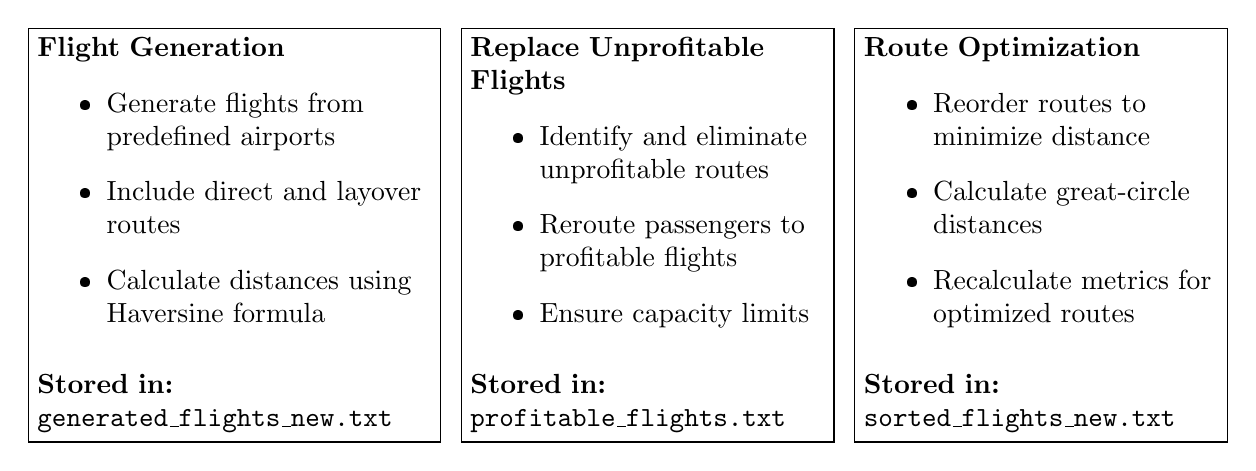
\begin{tikzpicture}[node distance=0.25cm, auto]
        % Node definitions
        \node (A) [draw, align=left, text width=5cm] {
            \textbf{Flight Generation}
            \begin{itemize}
                \item Generate flights from predefined airports
                \item Include direct and layover routes
                \item Calculate distances using Haversine formula
            \end{itemize}
            \vspace{0.2cm}
            \textbf{Stored in:}
            \texttt{generated\_flights\_new.txt}
        };

        \node (B) [draw, align=left, text width=4.5cm, right=of A] {
            \textbf{Replace Unprofitable Flights}
            \begin{itemize}
                \item Identify and eliminate unprofitable routes
                \item Reroute passengers to profitable flights
                \item Ensure capacity limits
            \end{itemize}
            \vspace{0.2cm}
            \textbf{Stored in:}
            \texttt{profitable\_flights.txt}
        };
        
        \node (C) [draw, align=left, text width=4.5cm, right=of B] {
            \textbf{Route Optimization}
            \begin{itemize}
                \item Reorder routes to minimize distance
                \item Calculate great-circle distances
                \item Recalculate metrics for optimized routes
            \end{itemize}
            \vspace{0.2cm}
            \textbf{Stored in:}
            \texttt{sorted\_flights\_new.txt}
        };
        
    \end{tikzpicture}
\end{frame}

%------------------------------------------------
\section{Flight Generator}
%------------------------------------------------

\begin{frame}{Flight Generation}
   \begin{minipage}{0.45\textwidth}
        \centering
        \includegraphics[width=\textwidth]{images/Screenshot from 2024-07-31 16-20-31.png}
        \caption{Output within\texttt{generated\_flights\_new.txt}}
    \end{minipage}
    \hfill
 
\end{frame}
%------------------------------------------------
\section{Sorting Flight Path}
%------------------------------------------------

\begin{frame}{Theorem}
    \begin{theorem}[Mass--energy equivalence]
        $E = mc^2$
    \end{theorem}
\end{frame}

%------------------------------------------------
\section{Remove and Replace Bad Flights}
%------------------------------------------------

\begin{frame}{Figure}
    Uncomment the code on this slide to include your own image from the same directory as the template .TeX file.
    %\begin{figure}
    %\includegraphics[width=0.8\linewidth]{test}
    %\end{figure}
\end{frame}

%------------------------------------------------
\section{Results}
%------------------------------------------------

\begin{frame}[fragile] % Need to use the fragile option when verbatim is used in the slide
    \frametitle{Citation}
    An example of the \verb|\cite| command to cite within the presentation:\\~

    This statement requires citation \cite{p1}.
\end{frame}

%------------------------------------------------
\section{Why}
%------------------------------------------------


%------------------------------------------------
\section{Conclusion}
%------------------------------------------------

\begin{frame}
    \Huge{\centerline{The End}}
\end{frame}

%------------------------------------------------
\section{References}
%------------------------------------------------

\begin{frame}{References}
    % Beamer does not support BibTeX so references must be inserted manually as below
    \footnotesize{
        \begin{thebibliography}{99}
            \bibitem[Smith, 2012]{p1} John Smith (2012)
            \newblock Title of the publication
            \newblock \emph{Journal Name} 12(3), 45 -- 678.
        \end{thebibliography}
    }
\end{frame}

\end{document}